%%=====================================================================================
%%
%%       Filename:  solution_assignment8_9.tex
%%
%%    Description:  Solution to assignment 8 and 9.
%%
%%        Version:  1.0
%%        Created:  04/10/2017
%%       Revision:  none
%%
%%         Author:  Dilawar Singh (), dilawars@ncbs.res.in
%%   Organization:  NCBS Bangalore
%%      Copyright:  Copyright (c) 2017, Dilawar Singh
%%
%%          Notes:  
%%                
%%=====================================================================================

\documentclass[a4paper,10pt]{article}
\usepackage{pgf,tikz,pgfplots}
\usepackage{amsmath}
\usepackage{amssymb}
\usepackage{chemfig}
\usetikzlibrary{shapes,backgrounds,decorations,decorations.pathmorphing}
\usetikzlibrary{calc,positioning}
% Title Page
\title{Title here} 
\author{Dilawar Singh}
\date{\today}
\begin{document}
\maketitle

\paragraph{Problem 8.1, 5 Points}

Supposing you had just two opsins in your retina, for red and blue, that drive
activity in red-selective and blue-selective neurons. Recall that the wavelength
curve for these is quite broad, and let us say that the curves overlap.  Draw a
graph with response on the y axis, and stimulus wavelength on the x axis, for
the two neurons.

\paragraph{Solution} The response curve of these two neurons to the light is
shown below. These are well approximated by following functions $blue(x) =
\exp\left( \frac{-(x-450)^2}{500}\right)$, and $red(x) = \exp\left(
\frac{-(x-550)^2}{2000}\right)$. Notice that these functions are also used to
approximate Dirac delta function.


\begin{tikzpicture}[scale=1]
    \begin{axis}[
            xlabel=Wavelength (nm),ylabel=Response
        , grid style={draw=gray!20}, grid = both
        , no markers
        , xmin = 400, xmax = 700
    ]
    \addplot gnuplot [ raw gnuplot ] {
            set xrange [400:800];
            blue(x)=exp( 20e-4 * -(x-450)^2 );
            plot blue(x) with lines;
    };
    \addplot gnuplot [ raw gnuplot ] {
            set xrange [400:800];
            red(x)=exp( 5e-4 * -(x-550)^2 );
            plot red(x) with lines;
    };
    \end{axis}
\end{tikzpicture}

\paragraph{Problem 8.2, 3 Points}
Consider the response of the red and blue neurons to a monchromatic yellow
stimulus, that has its wavelength 75\% closer to red than to blue. Come up with a
two-colour stimulus that would fool you into thinking it was the same colour as
yellow.

\paragraph{Solution} With values in previous solution, the wavelength is 525 nm.
At this wavelength the overall response is $blue(525) = 0.000013$ and $red(525)
= 0.7316$. The combination of both is roughly 0.7316. The problem is to find
$x$ and $y$ such that $blue(x)+red(x) + blue(y) + red(y) = 0.7316$. 
There are many solutions to this equation. One such solution is $x = 425$ and
$y=590$.

\paragraph{Problem 8.3, 5 Points}
Consider how inputs to a neuron sum, when they are located on an excitable
dendrite. On the x axis draw the number of converging active inputs, and on the
y axis draw the somatic excitation. Consider first summation if the inputs are
far below dendritic action-potential threshold (relatively few inputs), and then
draw what happens to somatic excitation as the number of inputs increases.

\paragraph{Solution} I made a approximate model for this problem and computed
the response at soma with varying N. Soma is far away from dendrite receiving
inputs (50 a.u. away). All inputs are 60 +/- 10 a.u. away from soma. The
time-difference between inputs are uniform random number 0 to 10 a.u. of time.
For totally synchronous input, this time-difference should be 0. Some results
are shown below. 

\includegraphics[width=0.4\textwidth]{./prob83_N10.png} 
\includegraphics[width=0.4\textwidth]{./prob83_N25.png}
\includegraphics[width=0.4\textwidth]{./prob83_N100.png}
\par

\includegraphics[width=0.4\textwidth]{./prob83_N125.png}
\includegraphics[width=0.4\textwidth]{./prob83_N398.png}
\includegraphics[width=0.4\textwidth]{./prob83_N1000.png}

If my model is correct, you were suppose to capture the following effect,
qualitatively or quantitatively.

\includegraphics[width=.8\textwidth]{./prob83_N_final.png}


\paragraph{Problem 8.4, 5 Points}
Design receptors and thresholds, for a set of 5 single neurons that can  do the
logical operations AND, OR, NOR, NAND and XOR, respectively. Assume only two
inputs in each case, A, and B. Explain how the last two work.

\paragraph{Solution} 


\tikz {  
    \node[] (a) {A};
    \node[below=of a] (b) {B};
    \node[right=of $(a)!0.5!(b)$,fill=blue!20] (x) {$\theta = w_1 + w_2 - \epsilon $ };
    \node[right=of x] (o) {A \texttt{AND} B};
    \draw[->] (a) to[ ] node[above, midway] {$w_1$} (x);
    \draw[->] (b) to[ ] node[above, midway] {$w_2$} (x);
    \draw[-] (x) -- (o);
}

\tikz {  
    \node[] (a) {A};
    \node[below=of a] (b) {B};
    \node[right=of $(a)!0.5!(b)$,fill=blue!20] (x) {$\theta = min(w_1, w_2) - \epsilon $ };
    \node[right=of x] (o) {A \texttt{OR} B};
    \draw[->] (a) to[ ] node[above, midway] {$w_1$} (x);
    \draw[->] (b) to[ ] node[above, midway] {$w_2$} (x);
    \draw[-] (x) -- (o);
}

\tikz {  
    \node[] (a) {A};
    \node[below=of a] (b) {B};
    \node[right=of $(a)!0.5!(b)$,fill=blue!20] (x) {$\theta = - \epsilon $ };
    \node[right=of x] (o) {A \texttt{NOR} B};
    \draw[->] (a) to[ ] node[above, midway] {$-w_1$} (x);
    \draw[->] (b) to[ ] node[above, midway] {$-w_2$} (x);
    \draw[-] (x) -- (o);
}

\tikz {  
    \node[] (a) {A};
    \node[below=of a] (b) {B};
    \node[right=of $(a)!0.5!(b)$,fill=blue!20] (x) {$\theta = max(-w_1,-w_2) - \epsilon $ };
    \node[right=of x] (o) {A \texttt{NAND} B};
    \draw[->] (a) to[ ] node[above, midway] {$-w_1$} (x);
    \draw[->] (b) to[ ] node[above, midway] {$-w_2$} (x);
    \draw[-] (x) -- (o);
}

This is bit odd!

\tikz {  
    \node[] (a) {A};
    \node[below=of a] (b) {B};
    \node[right=of $(a)!0.5!(b)$,fill=blue!20] (x) {$w_1 < \theta < -w_2 + \epsilon $ };
    \node[right=of x] (o) {A \texttt{XOR} B};
    \draw[->] (a) to[ ] node[above, midway] {$w_1$} (x);
    \draw[->] (b) to[ ] node[above, midway] {$-w_2$} (x);
    \draw[-] (x) -- (o);
}


\paragraph{Problem 9.1, 3 Points}

Read up how dopamine encodes reward expectation. In which of the situations will
you get the highest peak of dopamine? Explain why.

\begin{enumerate}
    \item Passing your course.
    \item Passing your course if you didn’t even study.
    \item Passing your course on the second attempt.
    \item Discovering that you had forgotten to register for the course so you don’t
even have to sit for the exam.

\end{enumerate}

\paragraph{Solution} Dopamine is released when there is an unexpected reward or
when one is thinking of reward in future. Essentially if you get a reward
without doing anything (or much), dopamine is released. I think 2 and 4 falls
into this category.

\paragraph{Problem 9.1, 5 Points}
Put together a few (named) signaling pathways to perform the operation of a NAND
gate, triggered by receptor activation, and using the activity of a kinase as
output. Which rate constants would you change to make it a NOR gate?

\paragraph{Solution} Recall that a NAND gate with inputs A and B, is ON when at
most 1 of the inputs is ON. Or in other words, if both A and B are ON, the
output is OFF, otherwise it is ON. The kinase has to be OFF when both signal are
high, and ON otherwise.

Let's say we have chemical species A and B (as input to gate), receptor R to
activate kinase X. Following is one solution:

\schemestart A + B \arrow{->[$k_1$]} AB \schemestop

\schemestart R + X \arrow{->[$k_2$]} $X^*$ + R \schemestop

\schemestart $X^*$ + AB \arrow{<->>[$k_f$][$k_b$]} XAB \schemestop

You need to find a signaling pathway which can do the above computation. Here is
the simulation of this scheme. When both A and B are zero, the system is high
(yellow). 

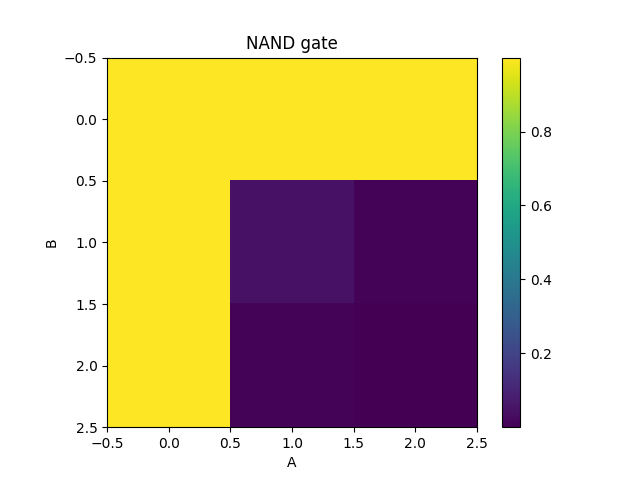
\includegraphics[width=0.7\textwidth]{./nand.png}

In this reaction scheme, we can not convert this gate to NOR gate by merely
changing the reaction rate.

\end{document}          

